\documentclass{beamer}

\usepackage[T2A]{fontenc}
\usepackage[utf8]{inputenc}
\usepackage[english,russian]{babel}
\usepackage{amssymb,amsfonts,amsmath,mathtext}
\usepackage{cite,enumerate,float,indentfirst}

\usepackage{graphicx}
\usepackage{booktabs}
\usepackage{tabularx}

\usepackage{qtree}    % regular trees (e.g. GB style)
\usepackage{gb4e}     % numbered lists for linguistic examples

\usepackage{caption}
\captionsetup{font=scriptsize}

\graphicspath{{images/}}

\usetheme{Rochester}
\usecolortheme{seagull}

\setbeamertemplate{footline}{\scriptsize{\hspace*{0.4cm}\insertframenumber}\vspace*{0.3cm}}
\beamertemplatenavigationsymbolsempty

\errorcontextlines 10000

\begin{document}

\title{\large{\sc Формальное моделирование}}
\author{Константин Соколов}

\begin{frame}
    \thispagestyle{empty}
    \titlepage
\end{frame}


\begin{frame}{}
\begin{center}
	\textbf{Вопрос для повторения}
\end{center}
\end{frame}

\begin{frame}{}
\begin{figure}[H]
	
\includegraphics[width=0.8\textwidth]{oil.jpg}
	\caption*{Кто победит?}
\end{figure}
\end{frame}

\begin{frame}{}
\begin{center}
	\textbf{$X'$-теория}
\end{center}
\end{frame}

\begin{frame}{Факт существования частей речи}
Различные морфологические и синтаксические свойства:\\
\medskip
\begin{exe}
	\ex различные парадигмы словоизменения
	    \begin{xlist}
		    \ex[]{дом, дома, дому, дом, домом, доме}
            \ex[]{иду, идёшь, идёт}
            \ex[]{понимай} 
        \end{xlist}
    \ex различная дистрибуция
	    \begin{xlist}
		    \ex[]{to drink water}
            \ex[]{to water the flowers}
        \end{xlist}
\end{exe}
\end{frame}

\begin{frame}{Факт существования синтаксических групп (I)}
Допустимость топикализации:\\
\medskip
\begin{exe}
	\ex глагольная группа
	    \begin{xlist}
            \ex[]{Он не способен \textit{совершить такую подлость}.}
		    \ex[]{\textit{Совершить такую подлость} он не способен.}
        \end{xlist}
	\ex именная группа
	    \begin{xlist}
            \ex[]{Я очень давно не видел \textit{Ивана}.}
		    \ex[]{\textit{Ивана} я очень давно не видел.}
        \end{xlist}
	\ex предложная группа
	    \begin{xlist}
            \ex[]{Нельзя ничего класть \textit{на этот стол}.}
		    \ex[]{\textit{На этот стол} нельзя ничего класть.}
        \end{xlist}
\end{exe}
\end{frame}

\begin{frame}{Факт существования синтаксических групп (II)}
Возможность замещения местоимением:\\
\medskip
\begin{exe}
    \ex 
	    \begin{xlist}
		    \ex[]{Что вы скажете об \textit{этом человеке, который предлагал нашей фирме очень выгодную операцию с ценными бумагами}?}
            \ex[]{Я скажу, что \textit{он} жулик.}
        \end{xlist}
    \ex[*]{Что вы скажете об этом \textit{нём}, который предлагал нашей \textit{ей} очень выгодную \textit{её} с \textit{ними}?}
\end{exe}
\end{frame}

\begin{frame}{Факт существования внутренней структуры группы}
\begin{exe}
    \ex 
	    \begin{xlist}
		    \ex[]{What are you going to do?}
            \ex[]{Help you.}
        \end{xlist}
	\ex {\small вершину группы нельзя удалить}
	    \begin{xlist}
		    \ex[]{I am trying to \textit{help you}.}
            \ex[]{I am trying to \textit{help}.}
            \ex[*]{I am trying to \textit{you}.}
        \end{xlist}
	\ex {\small нельзя заменить группой другого класса (NP на VP)}
	    \begin{xlist}
		    \ex[]{\textit{You} are difficult.}
            \ex[]{\textit{Help you} are difficult.}
        \end{xlist}
\end{exe}
\end{frame}

\begin{frame}{Факт единообразия структуры групп различных классов}
Сходные механизмы расширения групп:\\
\medskip
\begin{itemize}
    \item[NP:]{дом, большой дом, дом мельника, большой дом мельника, большой и красивый дом старого мельника}
    \item[VP:]{прятался, прятался в траве, часто прятался, часто прятался в зелёной траве}
    \item[AP:]{довольный, довольный собой, очень довольный собой, очень довольный собой и успехами своих детей}
    \item[PP:]{после дождя, после дождя в четверг, вскоре после холодного осеннего дождя, вскоре после непродолжительного дождя в четверг}
\end{itemize}
\end{frame}

\begin{frame}{Вывод}
\begin{quote}
``Предложение не составляется непосредственно из слов как из конститутивных элементов и не разложимо непосредственно на слова.''
\end{quote}
\begin{flushright}
\textit{{\small Золотова (1981), цит. по Тестелец (2001), стр. 144}}
\end{flushright}
\end{frame}

\begin{frame}[fragile]{$X'$-теория (базовая структура)}
Существует базовая структура группы:\\
\bigskip
\Tree [.XP [.Spec ] [.X' [.Adjunct ] [.X' [.X^0 ] [.Complement ] ] ] ]\\
\bigskip
Терминология: спецификатор, адъюнкт, вершина $X^0$, комплемент, первая проекция вершины $X'$, вторая (максимальная) проекция вершины $X'' = XP$, фразовая категория (``класс группы'')
\end{frame}

\begin{frame}[fragile]{$X'$-теория (вершина и комплемент)}
\begin{center}
\Tree [.NP [.N^0 портрет ] \qroof{короля Испании}.NP ]
\Tree [.VP [.V^0 бежать ] \qroof{на крышу}.PP ]\\
\medskip
\Tree [.PP [.P^0 после ] \qroof{выступления}.NP ]
\Tree [.AP [.A^0 сердитый ] \qroof{на весь мир}.NP ]
\end{center}
\end{frame}

\begin{frame}[fragile]{$X'$-теория (спецификатор и адъюнкт)}
\begin{center}
\Tree [.NP [.Spec мой ] [.N' [.N^0 дом ] ] ]
\Tree [.PP [.Spec сразу ] [.P' [.P^0 после ] \qroof{дождя}.NP ] ]
\Tree [.AP [.Spec очень ] [.A' [.A^0 сердитый ] \qroof{на весь мир}.PP ] ]
\end{center}
\end{frame}

\begin{frame}[fragile]{$X'$-теория (параметр расположения вершины)}
\begin{center}
\Tree [.XP [.Spec ] [.X' [.X^0 ] [.Compl ] ] ]
\Tree [.XP [.Spec ] [.X' [.Compl ] [.X^0 ] ] ]
\end{center}
\medskip
\begin{exe}
	\ex 
		\gll teburu-no ue-ni aru hon-o kure!\\
             стол.GEN на.LOC находящийся книга.ACC дай\\
		\glt \textit{дай книгу, которая лежит на столе!}
\end{exe}	
\end{frame}

\begin{frame}[fragile]{$X'$-теория (объяснительная сила)}
\begin{itemize}
	\item любая группа обладает вершиной, грамматические свойства вершины определяют свойства всей группы (принцип эндоцентричности)
	\item любой элемент синтаксической структуры является либо вершиной группы, либо проекцией вершины
	\item параметр расположения вершины позволяет объяснить явления правого и левого ветвления
\end{itemize}
\end{frame}


\begin{frame}{}
\begin{center}
	\textbf{Дискуссии}
\end{center}
\end{frame}

\begin{frame}{И. А. Мельчук vs. Я. Г. Тестелец (I)}
\begin{center}
        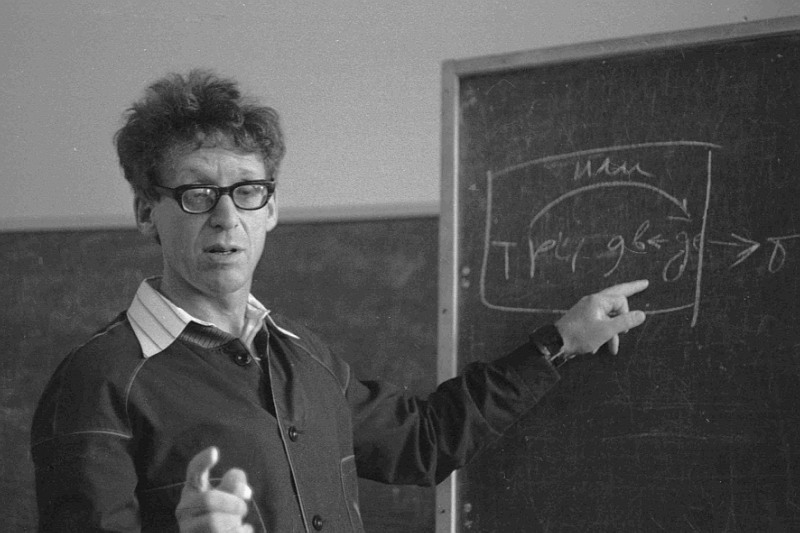
\includegraphics[width=0.506\textwidth]{melcuk.jpg}
        \hfill
        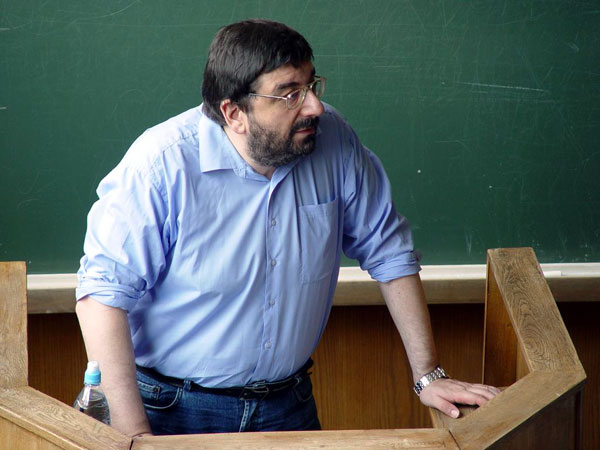
\includegraphics[width=0.45\textwidth]{testelets.jpg}
\end{center}
\end{frame}

\begin{frame}{И. А. Мельчук vs. Я. Г. Тестелец (II)}
\ \\
{\small <<Функциональная модель X предмета или явления Y -- это искусственно созданная система, быть может, совершенно иной физической природы, нежели Y, но такая, что если её поместить в обстановку, в которой действует Y, то она будет вести себя -- во всяком случае, в интересующем нас аспекте! -- достаточно похоже на Y, а в идеале -- неотличимо от Y. \dots [В]нутреннее, структурное тождество X-а и Y-а всё равно не гарантировано. [\dots] ``Создание модели есть доказательство ясности понимания.'' (Miller, Gallanter, Pribram 1960)>> \textit{(И.~А.~Мельчук, МСТ, с. 11-12)}}\\
\end{frame}

\begin{frame}{И. А. Мельчук vs. Я. Г. Тестелец (III)}
\ \\
{\small <<Есть объекты, которым мы нашли применение. Мы используем их, хотя почти наверняка не так, как их используют пришельцы. Я совершенно уверен, что в подавляющем большинстве случаев мы забиваем микроскопами гвозди.>> \textit{(А. и Б. Стругацие, ``Пикник на обочине'')}}\\
\end{frame}


\begin{frame}{}
    \thispagestyle{empty}
    \begin{center}
        {\large Спасибо!}
    \end{center}
\end{frame}


\end{document}
